\documentclass{standalone}
\usepackage{tikz}
\usepackage{ctex,siunitx}
\usepackage{tkz-euclide}
\usepackage{amsmath}
\usetikzlibrary{patterns, calc}
\usetikzlibrary {decorations.pathmorphing, decorations.pathreplacing, decorations.shapes,}
\begin{document}
\small
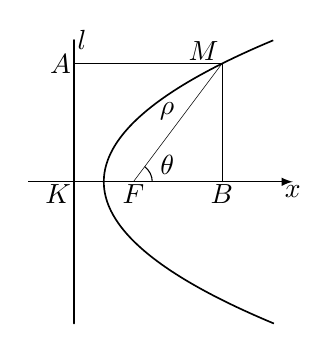
\begin{tikzpicture}[>=latex,scale=1.2,inner sep=1pt]
  \draw[thin,->](-0.8,0)--(2.0,0)node[below]{$x$};
  \tkzDefPoints{0/0/O,0.3125/0/F,-0.3125/0/K,1.25/1.25/M,-0.3125/1.25/A,1.25/0/B}
  \draw[semithick,domain=-1.5:1.5,samples=200] plot ({0.8*\x*\x},{\x});
  \tkzDrawSegments(M,A M,F M,B)
  \tkzLabelPoints[above left](M)
  \tkzLabelPoints[below](F,B)
  \tkzDrawLine[semithick,add=0.2 and 1.2](A,K)
  \tkzLabelLine[pos=-0.2,right](A,K){$l$}
  \tkzLabelLine[pos=0.5,above left](M,F){$\rho$}
  \tkzMarkAngle[size=0.2](B,F,M)
  \tkzLabelAngle[pos=0.4](B,F,M){$\theta$}
  \tkzLabelPoints[below left](K)
  \tkzLabelPoints[left](A)
\end{tikzpicture}
\end{document}